%-------------------------------
\section{Domain decomposition}
If we want to use more than one node of a cluster, we have to divide our problem into pieces.
%
In reservoir simulation, these pieces are called domains and they represented physical parts of the reservoir.
%
With domain decomposition we have a total parallel application, in this way we can estimate an upper limit we can reach without domain decomposition.
%
But each domains need to communicate part of their computation in order to solve the complete problem.

\section{Why did we have this problem ?}
At this point, the threaded part of the program doesn't know nothing about communications between processes.
%
So, communications can only happen in non-threaded part.
%
This is a problem because this make create synchronization  

\section{Create algorithm by assembling computation part}

\begin{figure}[!ht]
	\begin{center}
		\subfigure[Befor algorithm optimization]{%
			\label{fig:fusion_before}
			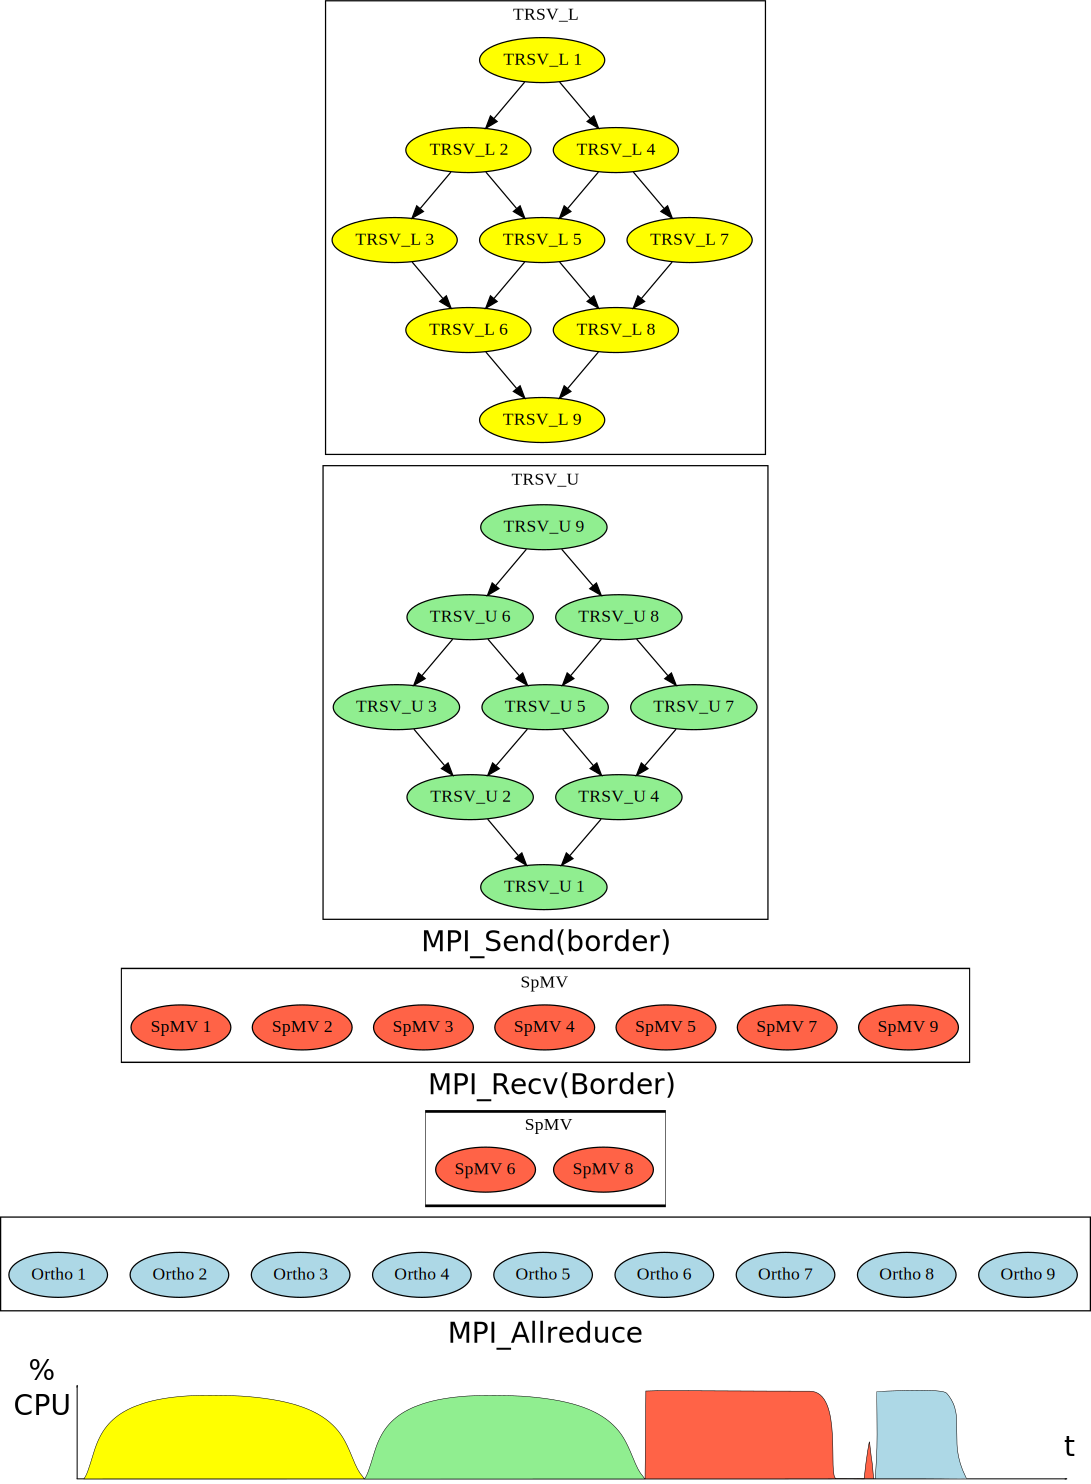
\includegraphics[width=0.49\textwidth]{fusion_before}
		}%
		\subfigure[After algorithm optimization]{%
			\label{fig:fusion_after}
			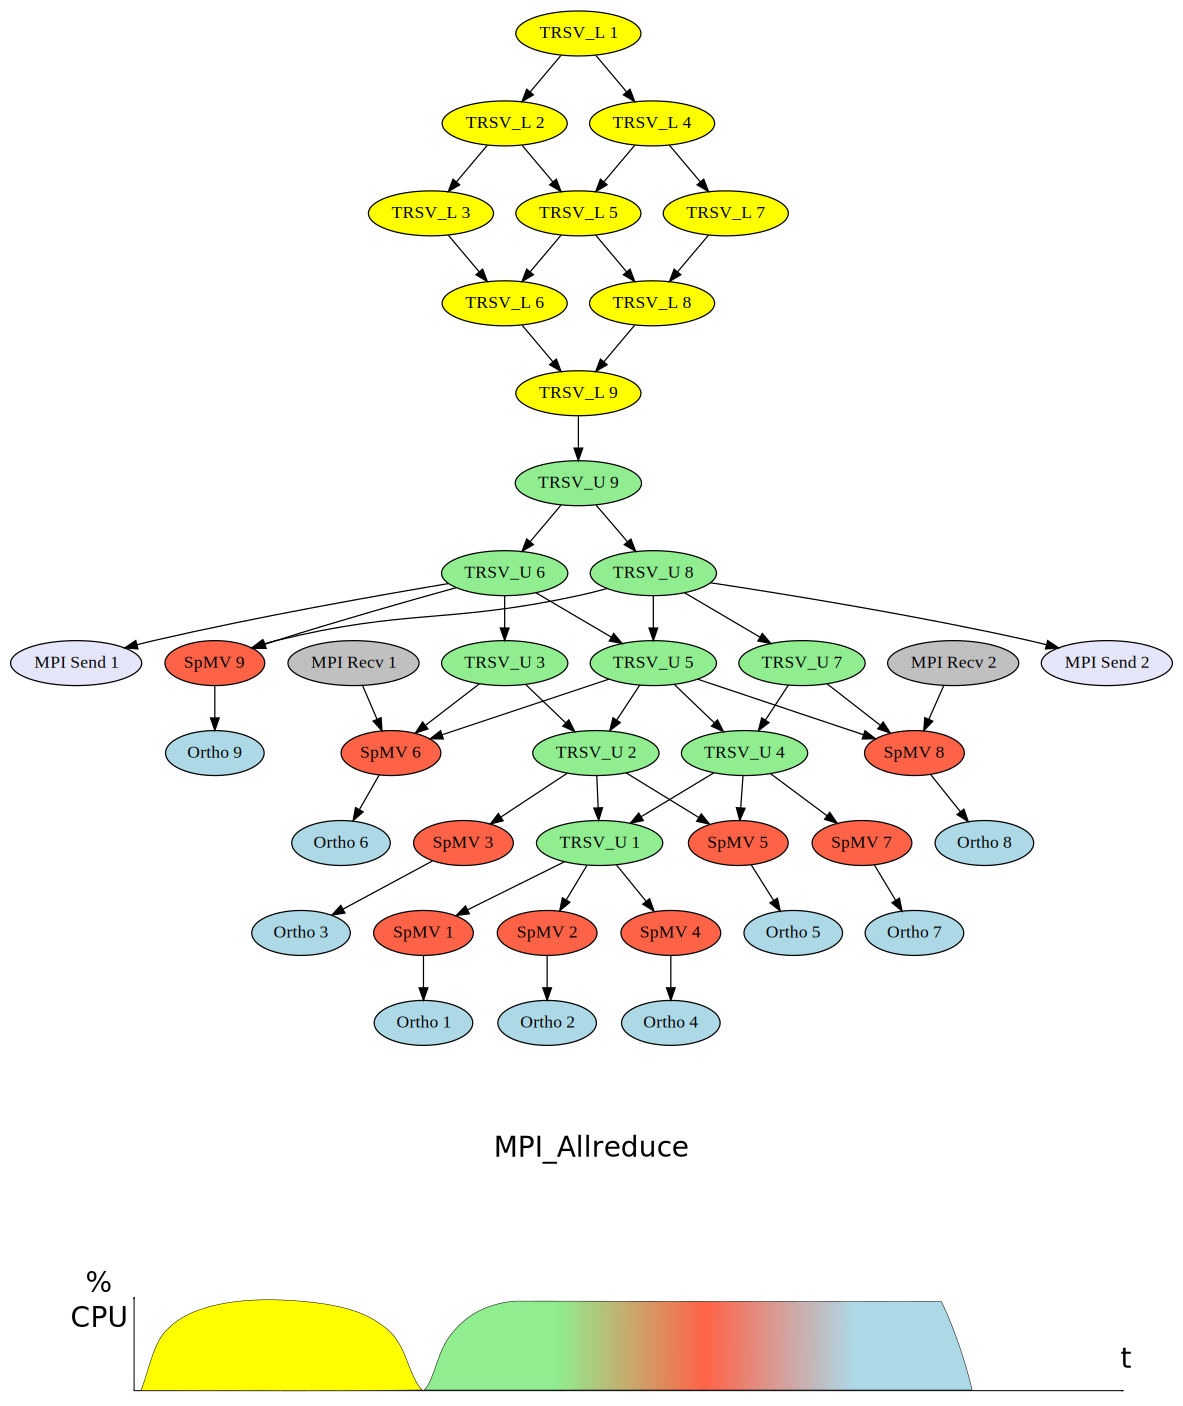
\includegraphics[width=0.49\textwidth]{fusion_after}
		}%
	\end{center}
	\caption{Example of fusion for preconditioned ILU GMRES.}
	\label{fig:fusion}
\end{figure}


\section{Result}
Good, I hope.
